\chapter{Описание предметной области и анализ существующих решений}

\section{Дерево принятия решений}

Дерево принятия решений (\texttt{Decision Tree}) --- модель применяющаяся
в алгоритмах машинного обучения, цель которой состоит в том, чтобы предсказать
значение целевой функции в заданной точке. Структура представляет собой
подвешенное дерево (часто двоичное), где в каждой вершине происходит разбиение
пространства по одному и признаков. Тем самым спускаясь по дереву до листа,
находится в какой области лежит заданная точка (лист дерева соответствующий
данной области), после чего возвращается значение функции в полученном листе
дерева.

Существуют различные алгоритмы для построения дерева, такие как: ID3, C4.5, CART
и другие. Обычно применяется построение сверху вниз, где на каждом шаге
происходит разбиение пространства по некоторому признаку, таким образом чтобы
максимизировать значение выбранной метрики. Часто применяющиеся метрики включают
себя: критерий Джини, информационный выигрыш и понижение дисперсии. Для избежания
переобучения, в конце работы алгоритма используется отсечение ветвей.

Преимуществами деревьев принятия решения по сравнению с другими моделями
машинного обучения являются:

\begin{enumerate}
    \item Понятная человеку интерпретация процесса принятия решения.
    \item Независимость от характера признаков --- может одинаково работать как
    целочисленными и вещественными признаками, так и с категориальными.
    \item Эффективная скорость обучения, даже при большом наборе данных.
\end{enumerate}

\section{Случайный регрессионный лес}

\begin{figure}[ht!]
\caption{Разбиение пространства случайным лесом}\label{random_forest}
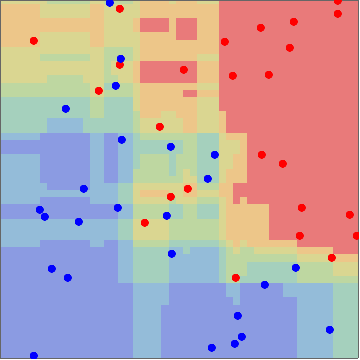
\includegraphics[height=0.35\textheight]{random_forest.png}
\end{figure}

Случайный лес (\texttt{Random Forest}\cite{randomforest}) --- модель машинного
обучения, основанная на применении ансамбля деревьев принятия решения, где
каждое дерево обучается независимо от остальных. Итоговый результат получается
как среднее (взвешенное среднее) по все ответам отдельных деревьев. Так как
каждое дерево разбивает пространство на прямоугольные области, где оно
возвращает одинаковые значения, то итоговый лес является пересечением всех таких
разбиений (Рисунок~\ref{random_forest}). Случайный лес называется регрессионным,
если он используется для решения задач предсказания некоторого численного
значения.

Для обучения регрессионного леса, исходные входные данные разбиваются на случайные
подвыборки с повторениями. После чего, на каждой выборке обучается отдельное
дерево принятия решений. Так же применяется метод \texttt{feature bagging}, где
деревья обучаются не на полном наборе признаков, а только на случено выбранном
его подмножестве.

\section{Постановка задачи}

В данной работе рассматривается задача оптимизации случайного регрессионного
леса.

Оптимизация --- задача нахождения экстремума (минимума или максимума) целевой
функци в некоторой области. Так как случайный лес разбивает пространство на
конечное число участков, то имеет место случай комбинаторной оптимизации.

Постановка Задачи: дан заранее обученный случайные лес. Необходимо найти области
пространства признаков в которых данный случайный лес возвращает свои
максимальное/минимальное значения.

\section{Существующие решения}

Так как функция задаваемая случайным лесом является трудно обратимой,
в настоящее время методы для её оптимизации не рассматривают внутреннюю
структуру случайного леса, а применяются общие методы для оптимизаций суррогатных
функции.

В данном случае основные подходы это:
\begin{enumerate}
    \item Случайный поиск --- выдирается случайная точка в пространстве,
    вычисляется значение функции в данной точке. Если полученный ответ лучше
    найденного ранее, то значение ответа обновляется.
    \item Локальный поиск --- поиск начинается из заданной точки, и на каждом шаге
    алгоритм переходит в соседнюю с лучшим значением оптимизируемой функции. Поиск
    останавливается при достижении локального экстремума или по истечении
    установленного времени.
\end{enumerate}

Также применяется комбинация этих двух алгоритмов, где производится локальный
поиск из набора случайных стартовых точек.

\section{Метод имитации отжига}

Популярным методом для решения задач оптимизации является метод имитации отжига.
Это общий алгоритмический метод решения задачи глобальной оптимизации, особенно
дискретной или комбинаторной. Основной идеей алгоритма, является имитация
физического процесса, происходящего при отжиге металлов, откуда алгоритм и берет
своё название.

Алгоритм производит случайные мутации по переходу из рассматриваемой точки
в соседнюю. При этом, переход в точку с худшим значением целевой функции
осуществляется с вероятностью, постепенно убывающей в соответствии с понижением
температуры:

\[
P(x_i \to x_{i+1}) =
\begin{cases}
    1,                                                  & F(x_i+1) > F(x_i) \\
    \exp \left(-\dfrac{F(x_{i+1})-F(x_i)}{T_i}\right),  & F(x_i+1) \geqslant F(x_i)
\end{cases}
\]

Где $P(x_i \to x_{i+1})$ --- вероятность события перехода в из точки $x_i$
в точку $x_{i+1}$. $F$ --- целевая функция. $T_i > 0$ --- убывающий
температурный параметр.

Основное преимущество данного алгоритма по сравнению с похожими методами
(локальный поиск) --- это случайность при переходе в следующее значение. Что
позволяет избегать остановки алгоритма в локальных экстремумах функции.

\section{Метод ветвей и границ}

Метод ветвей и границ (\texttt{branch and bound}) --- ещё один подход для
решения задач комбинаторной оптимизации. Основывается на методе полного
перебора, с отсечением тех вариантов, которые гарантированно не могут улучшить
найденное значение.

Основная идея метода заключается в том, что при некоторых ограничениях на
параметры целевой функции можно оценить её возможные значения. Тем самым можно
не перебирать те границы в которых гарантированно нет максимума функции, а те
границы в которых он потенциально может быть разбиваются на меньшие участки
и процесс повторяется.

Так как метод является вариацией полного перебора, то его эффективность сильно
зависит от качества оценки функции в заданных границах и правильного подбора
этих границ.

\chapterconclusion

В данной главе произведено теоретическое введение в модель машинного обучения
''случайный регрессионный лес''. Поставлена задача, решаемая в данной работе.
Также описаны и рассмотрены характеристики алгоритмов оптимизации, которые
используются на практике в данный монумент, и методы использованные в работе.
